\lecture{10}{11.08.2020}{Lyapunov Stability}

The major point we are concerned is how to assess the stability of a nonlinear system. That is, nonlinear analysis.

Nonlinear analysis is advantageous as linearization is an approximation and, therefor, valid only for small perturbations/signals.

To assess the stability, it is important to be able to prove mathematically/analytically that a given system remains stable under nonlinear behavior for large signals.

\subsection*{Definitions}

Given a not-necessarily-linear system \[
    \dot{x}(t) = f\left( x(t) \right) 
\] an equilibrium point $\overline{x}$ is a solution to \[
f\left( \overline{x}(t) \right) = 0 \forall t>\overline{t}
\]. An equilibrium point is calculated by solving \[
    f\left( \overline{x} \right) = 0
\] as it means that the derivative of the input is null and, therefore, the input achieves a constant value.

\begin{description}
    \item[Stability] is achieved if a given equilibrium point $\overline{x}$ if, for any perturbation of the system in a neighborhood of $\overline{x}$ results in a trajectory that remains in a finite neighborhood (epsilon-delta limit definition).
    \item[Asymptotical Stability] is achieved when it is stable and any resulting trajectory of neighbor perturbations of $\overline{x}$ converges to the equilibrium point (0).
\end{description}
Note that attractiveness does not imply stability.

\begin{figure}[H]
    \centering
    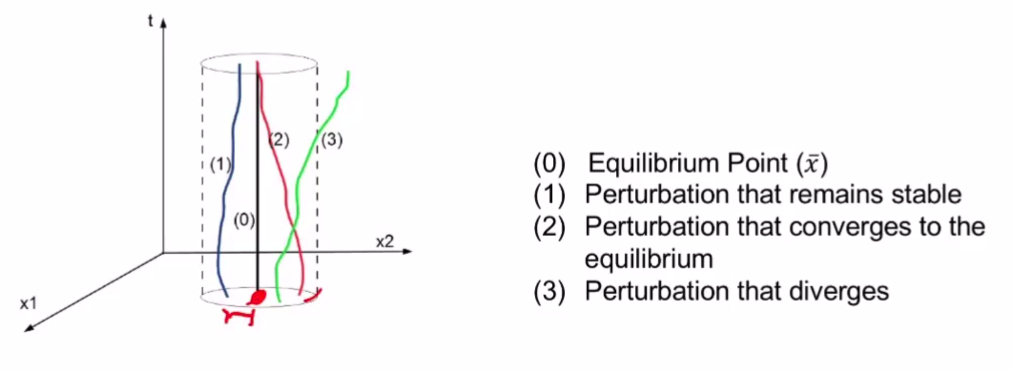
\includegraphics[width=0.8\textwidth]{figures/equilibrium_point.png}
    \caption{Equilibrium point demonstration. Note the axis.}
    \label{fig:figures-equilibrium_point-png}
\end{figure}

\subsection*{Lyapunov Method}

It consists in defining a scalar function $V\left( x \right) $ based on the state variables and to prove that this function is decreasing along the system trajectories. Based upon positive/negative definite function.

\begin{figure}[h!]
    \centering
    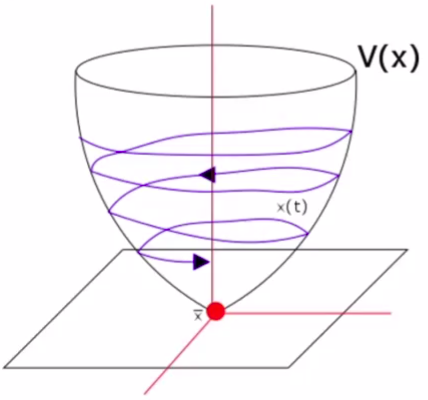
\includegraphics[width=0.8\textwidth]{figures/lyapunov_function.png}
    \caption{Lyapunov function illustrated.}
    \label{fig:figures-lyapunov_function-png}
\end{figure}

\begin{description}
    \item[Positive definite] is a function $V\left( x \right) :R^{n}\to R$ that, in a point $\overline{x}$ is guaranteed that $V\left( \overline{x} \right) =0$ and  $\exists \xi>0:V\left( x \right) >0 \forall x:\|x-\overline{x}\|<\xi$ when $x\neq \overline{x}$ (if we relax the restriction on the neighborhood of $\overline{x}$ to $V(x) \ge 0$, then this function is \textbf{semi positive-definite}).
    \item[Negative definite] is a function $V\left( x \right) :R^{n}\to R$ such that $-V(x)$ is \emph{positive definite}.
\end{description}

 Usually it is very difficult for nonlinear systems to prove behavior over the entire design space, so what is normally assessed is the region where perturbations develop towards the equilibrium point (attraction zone).

 Given a system $\dot{x}(t)=f\left( x(t) \right) $, we define a Lyapunov function $V\left( x \right) $ such that
\begin{itemize}
    \item $V$ is a \emph{positive-definite} function over $x$.
    \item $\frac{d}{dt}V\left( x \right) =\dot{V}\left( x \right)$ is \emph{(semi) negative-definite}.
	\begin{itemize}
	    \item if strictly negative-definite, then \emph{asymptotic stability} is achieved, that is, effectively an attraction zone.
	    \item if semi negative-definite, then some \emph{oscillations} will occur around the equilibrium point in the case of $\frac{d}{dt}V = 0$.
	\end{itemize}
\end{itemize}

% STOPPED BY 45:00
